\id{МРНТИ 06.75.13}{}

\begin{articleheader}
\sectionwithauthors{А.У. Кукетаева, Г.С. Муханова, А.Ж. Турегельдинова, А.К. Мустафина}{ЦИФРОВИЗАЦИЯ КАК ФАКТОР УСПЕХА УПРАВЛЕНИЯ ИТ-ПРОЕКТАМИ В КАЗАХСТАНЕ}

{\bfseries
\textsuperscript{1}А.У. Кукетаева\textsuperscript{\envelope },
\textsuperscript{1}Г.С. Муханова,
\textsuperscript{1}А.Ж. Турегельдинова,
\textsuperscript{2}А.К. Мустафина
}
\end{articleheader}

\begin{affiliation}
\textsuperscript{1}Satbayev University, Алматы, Казахстан,

\textsuperscript{2}Международный Университет информационных технологий, Алматы, Казахстан

\raggedright \textsuperscript{\envelope }Корреспондент-автор: asel.k@mail.ru
\end{affiliation}

На фоне стремительных изменений в сфере технологий цифровизация всё чаще
рассматривается как один из ключевых факторов, влияющих на успешное
управление ИТ-проектами. В казахстанском контексте особую роль в этом
процессе играет государственная программа «Цифровой Казахстан». Её
реализация способствует внедрению современных цифровых решений в
различные секторы экономики. Вместе с тем, на практике цифровизация
сопровождается рядом трудностей: ощущается нехватка профессиональных
кадров, наблюдается дисбаланс в развитии цифровой инфраструктуры между
регионами, а участие управленческого звена в цифровых инициативах
остаётся на низком уровне.

Цель проведённого исследования - понять, как цифровизация влияет на
эффективность управления ИТ-проектами в условиях Казахстана. В рамках
работы был организован опрос среди специалистов в области проектного
менеджмента, а для анализа данных использовались методы количественной
статистики, в том числе регрессионный анализ, ANOVA и хи-квадрат.
Результаты показали, что на уровень цифровизации существенно влияет
вовлечённость руководства - этот фактор оказался гораздо более значимым,
чем профессиональный опыт самих менеджеров проектов.

В итоге исследование подтверждает: без активной поддержки цифровых
инициатив на уровне руководства трудно рассчитывать на успешную
реализацию ИТ-проектов. Стратегическое участие управленцев способно
ускорить внедрение цифровых решений и повысить общую результативность
цифровой трансформации в Казахстане.

{\bfseries Ключевые слова:} цифровизация, ИТ-проекты, управление проектами,
Казахстан, цифровая \\трансформация, вовлеченность руководства,
эффективность проектов.

\begin{articleheader}
{\bfseries ҚАЗАҚСТАНДАҒЫ IT-ЖОБАЛАРДЫ БАСҚАРУДЫҢ ТАБЫСТЫ ФАКТОРЫ РЕТІНДЕ ЦИФРЛАНДЫРУ}

{\bfseries
\textsuperscript{1}Ә.У.Көкетаева\textsuperscript{\envelope },
\textsuperscript{1}Г.С.Муханова,
\textsuperscript{1}Ә.Ж.Төрегелдинова,
\textsuperscript{2}А.К.Мустафина
}
\end{articleheader}

\begin{affiliation}
\textsuperscript{1}Satbayev University, Алматы, Қазақстан,

\textsuperscript{2}Халықаралық ақпараттық технологиялар университеті, Алматы, Қазақстан,

e-mail: asel.k@mail.ru
\end{affiliation}

Технологиялық өзгерістердің қарқыны күннен-күнге артып келе жатқан
қазіргі жағдайда цифрландыру IT-жобаларды тиімді басқарудың негізгі
тетіктерінің бірі ретінде алға шығады. Қазақстанда бұл үдеріс «Цифрлық
Қазақстан» мемлекеттік бағдарламасы аясында жүзеге асырылып, ел
экономикасын жаңғыртуға және заманауи цифрлық шешімдерді енгізуге
айтарлықтай ықпал етуде. Алайда оң өзгерістерге қарамастан, цифрландыру
бірқатар өзекті мәселелермен бетпе-бет келіп отыр. Атап айтқанда, жоғары
білікті кадрлардың жетіспеушілігі, цифрлық инфрақұрылымның аймақтар
арасында тең дәрежеде дамымауы және басшылық деңгейінде цифрлық
бастамаларға жеткіліксіз қолдау көрсетілуі - бұл саланың дамуын тежейтін
басты факторлар ретінде көрініс табуда.

Осы зерттеу жұмысы Қазақстандағы цифрландырудың IT-жобаларды басқару
тиімділігіне нақты қандай әсер ететінін саралауға бағытталды. Жоба
менеджерлері арасында сауалнама жүргізіліп, алынған деректер негізінде
регрессиондық талдау, ANOVA және хи-квадрат секілді статистикалық
әдіс\-тер қолданылды. Нәтижелер көрсеткендей, ұйым басшылығының цифрлық
трансформация үдерісіне белсенді араласуы цифрландыру деңгейіне тікелей
ықпал етеді. Ал жобалық менеджерлердің кәсіби тәжірибесі жобаның
табысына шешуші әсер ете бермейтінін аңғартты.

Жүргізілген зерттеу негізінде ұйымдардағы цифрландыру бастамаларын
жоғарғы деңгейде қолдау қажеттігі анық байқалады. Бұл IT-жобалардың
нәтижелілігін арттыруға және Қазақстанда цифрлық өзгерістерді
жеделдетуге нақты мүмкіндік береді.

{\bfseries Түйін сөздер:} цифрландыру, IT-жобалар, жобаларды басқару,
Қазақстан, цифрлық трансформация, басшылықтың қатысуы, жобалық
тиімділік.

\begin{articleheader}
{\bfseries DIGITALIZATION AS A SUCCESS FACTOR IN IT PROJECT MANAGEMENT IN KAZAKHSTAN}

{\bfseries
\textsuperscript{1}A.U.Kuketayeva\textsuperscript{\envelope },
\textsuperscript{1}G.S.Mukhanova,
\textsuperscript{1}А.Zh.Turegeldinova,
\textsuperscript{2}A.K.Mustafina
}
\end{articleheader}

\begin{affiliation}
\textsuperscript{1}Satbayev University, Almaty, Kazakhstan,

\textsuperscript{2}IITU, Almaty, Kazakhstan,

e-mail: asel.k@mail.ru
\end{affiliation}

In today' s landscape of rapidly evolving technology,
digitalization has emerged as a significant factor contributing to the
success of IT project management. Within Kazakhstan, the \emph{Digital
Kazakhstan} initiative has taken on a central role in driving economic
transformation by enabling the adoption of cutting-edge digital tools
and systems. Nonetheless, despite considerable progress, the
digitalization journey continues to face a set of persistent challenges
--- notably, a lack of skilled professionals, disparities in digital
infrastructure across regions, and limited involvement of senior
management in digital transformation initiatives.

The purpose of this study is to explore how digitalization influences
the effectiveness of IT project management in Kazakhstan. To achieve
this, a survey was carried out targeting professionals in project
management roles, and a range of statistical methods were employed to
analyze the data - including regression analysis, ANOVA, and the
chi-square test. The findings reveal that the active participation of
management has a strong and measurable impact on the level of
digitalization achieved, whereas the length of experience held by
project managers does not appear to be a decisive factor.

Ultimately, the results highlight the importance of strategic engagement
from leadership teams in suppor\-ting digital initiatives. Strengthening
such support can improve the outcomes of IT projects and help accelerate
the broader digital transformation across Kazakhstan.

{\bfseries Keywords:} digitalization, IT project management, Kazakhstan,
digital transformation, leadership enga\-gement, project outcomes.

\begin{multicols}{2}
{\bfseries Введение}. На фоне стремительного технологического прогресса
цифровизация постепенно превращается в один из ключевых факторов,
обеспечивающих устойчивость и конкурентоспособность организаций в самых
разных сферах экономики. Сегодня успешная реализация ИТ-проектов
практически невозможна без внедрения цифровых решений - они позволяют
упростить внутренние процессы, повысить рациональность использования
ресурсов и наладить более эффективное взаимодействие между всеми
участниками проектов.

В казахстанских реалиях цифровизация получила статус одного из важнейших
национальных приоритетов. Это отражено в государственной программе
«Цифровой Казахстан», основная цель которой - не только ускорение темпов
экономического роста, но и улучшение повседневной жизни населения.
Программа охватывает широкий спектр направлений: от внедрения цифровых
технологий в ключевые отрасли экономики до развития цифровых компетенций
у граждан и создания современной инновационной инфраструктуры.

Тем не менее, несмотря на прикладываемые усилия, внедрение ИТ-проектов в
условиях цифровой трансформации сопровождается рядом существенных
трудностей. Наиболее остро ощущается нехватка специалистов с актуальными
цифровыми компетенциями, особенно в регионах, где развитие
инфраструктуры зачастую отстаёт от потребностей. Также стоит отметить
слабую интеграцию современных технологий в традиционные отрасли
экономики, а в ряде случаев - и отсутствие достаточной
нормативно-правовой базы, способной поддержать цифровые инициативы. Все
эти факторы затрудняют реализацию ИТ-проектов и тормозят общее
продвижение цифровизации.

Исследование данной темы представляется особенно важным в текущих
условиях, поскольку своевременное выявление и устранение подобных
барьеров может способствовать формированию более действенных подходов к
управлению ИТ-проектами. Это, в свою очередь, повысит их эффективность и
создаст условия для ускорения цифровых преобразований в Казахстане.

По своей сути цифровизация - это не просто внедрение технологий, а
комплексный процесс, охватывающий все уровни организационной
деятельности. Её задачи заключаются в том, чтобы повысить
производительность, упростить внутренние процедуры и обеспечить более
тесное взаимодействие между всеми участниками проектов. Особенно заметно
её значение в управлении ИТ-проектами, где всё чаще применяются цифровые
инструменты: автоматизированные системы, аналитические платформы и среды
для совместной работы. Эти решения позволяют ускорить планирование,
сделать контроль более прозрачным и упростить реализацию задач на каждом
этапе проекта.

На международной арене уже накоплен значительный опыт, демонстрирующий
преимущества цифровизации. Исследования показывают, что использование
таких технологий, как искусственный интеллект, блокчейн, облачные
платформы и системы анализа больших данных, существенно увеличивает
вероятность успешного завершения проектов. Эти инструменты становятся
неотъемлемой частью профессионального набора современного проектного
менеджера.

Понятие критических факторов успеха (Critical Success Factors, CSF)
охватывает ключевые условия, без которых трудно рассчитывать на
положительный исход ИТ-проектов. В условиях активной цифровой
трансформации к таким факторам всё чаще относят следующие элементы:


- наличие в организации чётко сформулированной цифровой стратегии;

- высокий уровень цифровой грамотности персонала;

- доступ к современным цифровым инструментам и платформам;

- эффективное управление изменениями, возникающими в процессе
цифровизации;

- активное участие и поддержка со стороны топ-менеджмента.

Существующие проектные подходы - такие как PRINCE2, PMBOK и Agile -
адаптируются к условиям цифровой среды, позволяя учитывать специфику
новых технологий и ускоряющихся процессов.

Практика в разных странах демонстрирует, что цифровизация способна
существенно повысить эффективность управления проектами. Ведущие
технологические компании, включая Amazon и Google, активно используют
цифровые инструменты и аналитические решения для планирования, контроля
и реализации своих проектов. В государствах с развитой цифровой
культурой, таких как Южная Корея и Сингапур, цифровые технологии стали
неотъемлемой частью бизнес-процессов, включая управление
ИТ-направлением. Для Казахстана изучение и адаптация таких успешных
кейсов может сыграть важную роль в ускорении собственной цифровой
трансформации.

Данная статья посвящена анализу того, как цифровизация влияет на
эффективность управления ИТ-проектами в Казахстане. Особое внимание
уделяется возможностям повышения результативности за счёт внедрения
цифровых подходов и инструментов.

В рамках поставленной цели были определены следующие задачи:

1. Рассмотреть теоретические основы цифровизации и её влияние на
проектное управление в ИТ-сфере.

2. Оценить текущий уровень цифровизации в Казахстане и его отражение на
ключевых элементах управления проектами.

3. Определить наиболее значимые факторы успеха ИТ-проектов, связанные с
цифровыми преобразованиями.

4. Разработать практические рекомендации для казахстанских компаний по
интеграции цифровых решений в проектную деятельность.

{\bfseries Литературный обзор.} В последние годы цифровизация стала одним
из ключевых факторов, влияющих на успешное управление ИТ-проектами в
Казахстане. Данная статья рассматривает основные направления и
результаты исследований в этой области. Программа «Цифровой Казахстан»,
утвержденная в 2017 году, направлена на ускорение темпов развития
экономики и улучшение качества жизни населения через использование
цифровых технологий. В рамках этой программы реализуются проекты,
ориентированные на развитие цифровой инфраструктуры, повышение цифровой
грамотности населения и внедрение инновационных решений в различных
отраслях экономики {[}1{]}. Цифровизация оказывает значительное влияние
на методы и подходы в управлении проектами.

В статье «Управление проектами в условиях цифровой трансформации
Казахстана» {[}2{]} рассматриваются изменения, происходящие в подходах к
управлению проектами в условиях активного внедрения цифровых технологий.
Авторы обращают внимание на то, что традиционные методы управления
требуют адаптации к новым условиям. Особый акцент сделан на
необходимости интеграции цифровых инструментов и платформ, что, по
мнению исследователей, способствует росту эффективности и гибкости
проектного управления.

В свою очередь, работа под названием «IT-услуги в Казахстане: динамика и
возможности цифровизации промышленности» {[}3{]} фокусируется на
развитии ИТ-сектора и его влиянии на промышленную цифровизацию. В ходе
анализа авторы приходят к выводу, что рост информационных и компьютерных
услуг создаёт благоприятную основу для дальнейшей цифровой трансформации
в промышленности. Тем не менее, несмотря на позитивную динамику, в
процессе цифровизации сохраняются определённые сложности. К числу
наиболее значимых проблем относятся дефицит квалифицированных ИТ-кадров,
необходимость обновления существующей инфраструктуры, а также
потребность в адаптации законодательных и регуляторных механизмов к
новым технологическим условиям.

В статье «Цифровизация через призму проектного управления» {[}4{]}
подчеркивается важность стратегического подхода и системного внедрения
цифровых технологий для преодоления указанных препятствий. В
исследовании «Оценка влияния информационных технологий на эффективность
государственного управления» {[}5{]} анализируются теоретические и
прикладные аспекты влияния ИТ на государственное управление.
Исследования подчёркивают, что грамотное применение информационных
технологий может значительно повысить как прозрачность, так и
результативность государственных процессов.

Так, в работе «Влияние цифровых технологий на экономику Казахстана»
{[}6{]} делается акцент на том, что цифровые решения играют
принципиально важную роль в сохранении национального суверенитета - как
в технологическом, так и в информационном аспекте. Авторы подчёркивают
необходимость активного и продуманного внедрения цифровых инструментов,
рассматривая это как основу для устойчивого экономического роста страны.

В другой публикации {[}7{]} рассматривается оригинальный подход к
проектному управлению: предлагается модель, в которой распределение
функций между цифровыми платформами и командой осуществляется более
гибко. Такой подход, по мнению авторов, повышает шансы на успешную
реализацию проектов в рамках цифрового менеджмента.

Авторы исследования {[}8{]} анализируют, как цифровая трансформация
влияет на организационные модели управления. Особое внимание они уделяют
тому, насколько важна чёткая структура и адаптивность в условиях
неопределённости, особенно на ранних стадиях проекта.

В статье {[}9{]} рассмотрен вопрос о том, как цифровизация и
стандартизация процессов могут положительно сказаться на качестве
выполнения проектов в различных отраслях. Авторы подчёркивают, что
именно сочетание этих подходов обеспечивает более высокую управляемость
и эффективность.

Обобщая имеющиеся публикации, можно заключить, что цифровизация
действительно оказывает серьёзное влияние на успешность управления
ИТ-проектами в Казахстане. Национальные программы и инициативы формируют
благоприятную среду для развития цифровых процессов. Однако, чтобы этот
потенциал реализовался в полной мере, необходимо преодолеть существующие
ограничения: улучшить инфраструктуру, закрыть кадровые пробелы и
привести нормативную базу в соответствие с требованиями времени.
Продолжение интеграции цифровых решений в практику управления остаётся
приоритетной задачей для устойчивого развития отрасли.

{\bfseries Материалы и методы.} В исследовании использовалась
онлайн-анкета. Опрос был анонимным и проводился в 2025 году
январь/февраль. Исследовательская группа была проектные менеджера
ИТ-проектов, с опытом работы более 3-х лет. Для сбора данных
использовался инструмент Google Forms. В течение месяца было собрано 31
полностью заполненных электронных опросов. Респондентов попросили
оценить представленные потенциальные элементы, влияющие на успех
проекта.

Респондентам было предложено ответить о своем последнем завершённом
ИТ-проекте. Анкета состояла из четырёх разделов и включала вопросы,
направленные на анализ влияния цифровизации на успешность управления
проектами.

Раздел 1. Общая информация о респонденте. Включал вопросы о
профессиональном опыте, отрасли работы и используемых методологиях
управления проектами.

Раздел 2. Влияние цифровизации на управление проектами.

Целью этого раздела было исследование степени цифровизации в
организациях и определение её влияния на ключевые аспекты проектного
управления. Опрос помог зафиксировать, как цифровые инструменты и
процессы внедряются на практике и насколько они помогают в достижении
проектных целей.

Раздел 3. Ключевые факторы успеха ИТ-проектов.

В этом блоке акцент был сделан на выявление наиболее значимых условий,
способствующих успешной реализации ИТ-проектов. Участникам опроса
предлагалось оценить влияние различных факторов, таких как доступ к
технологиям, квалификация персонала, управленческие подходы и поддержка
со стороны руководства.

Раздел 4. Заключительные вопросы.

Финальная часть анкеты включала открытые вопросы. Здесь респонденты
могли свободно выразить свои взгляды на основные сложности, с которыми
сталкиваются организации при цифровизации, и предложить конкретные пути
улучшения управления ИТ-проектами в условиях казахстанской реальности.

Собранные ответы легли в основу анализа взаимосвязей между уровнем
цифровой зрелости, управленческой поддержкой, профессиональной
подготовкой сотрудников и конечной результативностью ИТ-проектов.

Для обработки и интерпретации данных были использованы различные методы:
корреляционный анализ, SWOT-анализ, регрессионный анализ, а также
дисперсионный анализ (ANOVA), что позволило оценить статистическую
значимость выявленных зависимостей.\\
{\bfseries Гипотезы исследования:}

- H1: Высокая вовлеченность руководства {\bfseries положительно влияет} на
успешность управления ИТ-проектами.

- H2: Развитая цифровая инфраструктура {\bfseries способствует} успешному
внедрению цифровых технологий.

- H3: Квалификация ИТ-специалистов {\bfseries повышает} эффективность
управления ИТ-проектами.

- H4: Опыт проектного менеджера {\bfseries может усиливать} влияние
цифровых факторов на успех проектов.

Для статистической обработки данных была рассмотрена исследовательская
модель Рисунок 1.
\end{multicols}

\begin{figure}[H]
	\centering
	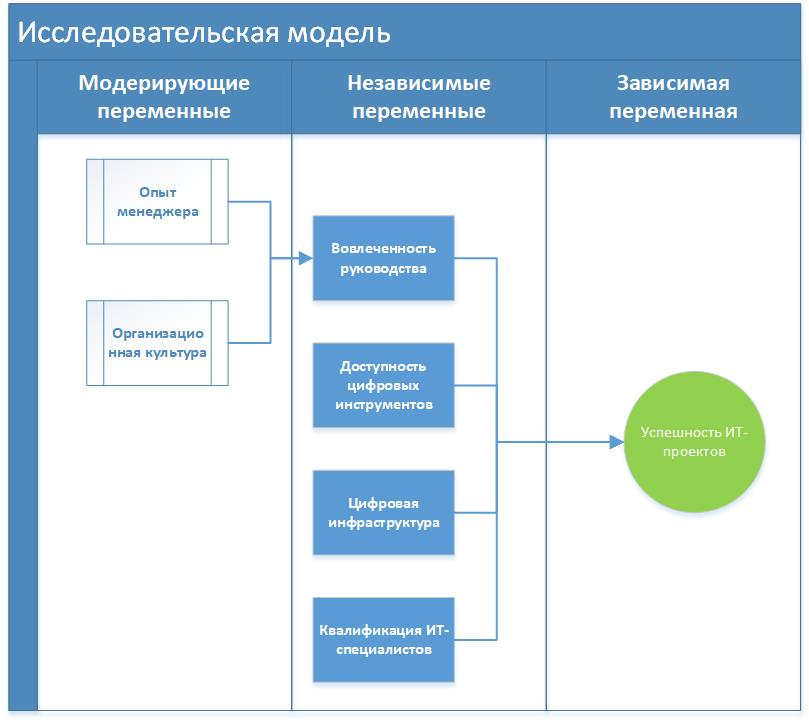
\includegraphics[width=0.6\textwidth]{media/ekon2/image47}
	\caption*{Рис.1 - Исследовательская модель}
    \caption*{\normalfont\emph{Примечание - Разработано авторами}}
\end{figure}

\tcap{Таблица 1 - «Регрессионный анализ»}
\begin{longtblr}[
  label = none,
  entry = none,
]{
  width = \linewidth,
  colspec = {Q[344]Q[246]Q[88]Q[256]},
  cells = {c},
  cell{6}{1} = {c=4}{0.933\linewidth},
  hlines,
  vlines,
}
Переменная & Бета-коэффициент
			(β) & p-value & Значимость\\
Вовлеченность
			руководства & 0.6607 & 0.0001 & Статистически
			значимо\\
Цифровая
			инфраструктура & 0.4213 & 0.003 & Статистически
			значимо\\
Квалификация
			ИТ-специалистов & 0.503 & 0.000 & Статистически
			значимо\\
Опыт
			менеджера & 0.189 & 0.213 & Не
			значимо\\
Примечание
			– Разработано авторами &  &  & 
\end{longtblr}

\begin{multicols}{2}
{\bfseries Обсуждение и результаты.} После обработки данных и проведения
статистического анализа (корреляционный анализ, регрессионный анализ,
ANOVA и хи-квадрат тест) мы можем сделать следующие выводы по каждой из
гипотез:

H1: Высокая вовлеченность руководства положительно влияет на успешность
управления ИТ-проектами. Подтверждено

Регрессионный анализ (Таблица 1) показал, что вовлеченность руководства
оказывает сильное положительное влияние на уровень цифровизации
(коэффициент корреляции 0.725, p-value \textless{} 0.001). Это означает,
что чем больше руководство поддерживает цифровизацию, тем выше
вероятность успешного завершения ИТ-проекта. Руководителям организаций
следует активно участвовать в процессах цифровизации, выделять ресурсы и
стратегически поддерживать ИТ-инициативы.

H2: Развитая цифровая инфраструктура способствует успешному внедрению
цифровых технологий - подтверждено.

Анализ показал, что уровень цифровизации напрямую связан с доступностью
технологических решений и качеством существующей инфраструктуры. Там,
где организации располагают современными цифровыми ресурсами, проекты в
сфере ИТ демонстрируют значительно лучшие результаты (p-value
\textless{} 0.05). Это подтверждает: для повышения эффективности
ИТ-проектов компаниям стоит уделить внимание обновлению цифровой
инфраструктуры, включая внедрение облачных сервисов, интернет-технологий
и автоматизированных платформ.

H3: Квалификация ИТ-специалистов влияет на эффективность управления
проектами - подтверждено.

Респонденты, обладающие более высокой цифровой компетентностью, как
правило, давали положительную оценку цифровизации в своих организациях.
В тех случаях, где уровень подготовки персонала оставался низким,
внедрение технологий сопровождалось затруднениями. Таким образом,
инвестиции в обучение сотрудников, развитие их цифровых навыков и
реализация программ повышения квалификации являются необходимыми
условиями для успешной цифровой трансформации.

H4: Опыт проектного менеджера усиливает влияние цифровых факторов на
успех проекта - не подтверждено.

Результаты корреляционного анализа (см. Таблицу 2) показали, что стаж
работы менеджера не оказывает существенного влияния на степень
цифровизации или успех проекта (p-value \textgreater{} 0.05). Как
опытные, так и менее опытные руководители демонстрировали схожие оценки.
При этом наибольшее значение имели вовлечённость руководства, качество
цифровой инфраструктуры и подготовленность специалистов. Следовательно,
хотя управленческий опыт остаётся важным, он не является определяющим
фактором в контексте цифровой трансформации.
\end{multicols}

\tcap{Таблица 2 - «Корреляционный анализ»}
\begin{longtblr}[
  label = none,
  entry = none,
]{
  width = \linewidth,
  colspec = {Q[398]Q[229]Q[73]Q[235]},
  cells = {c},
  cell{4}{1} = {c=4}{0.934\linewidth},
  hlines,
  vlines,
}
Переменные & Коэффициент
			корреляции (r) & p-value & Вывод\\
Вовлеченность
			руководства → Уровень цифровизации & 0.725 & 0.0001 & Сильная
			положительная связь\\
Опыт
			менеджера → Уровень цифровизации & 0.0387 & 0.8511 & Связь
			отсутствует\\
Примечание
			– Разработано авторами &  &  & 
\end{longtblr}

\begin{multicols}{2}
Подтверждены гипотезы H1, H2 и H3 - вовлеченность руководства, цифровая
инфраструктура и квалификация ИТ-специалистов значительно влияют на
успешность управления ИТ-проектами.

H4 (влияние опыта менеджера) не подтверждена - опыт не является решающим
фактором, а вовлеченность руководства играет более важную роль.

Результаты проведённого опроса показывают, что эффективность управления
ИТ-проектами в Казахстане во многом определяется уровнем цифровой
зрелости организаций, степенью вовлечённости и стратегическим видением
руководства, а также профессиональной подготовкой проектных команд. В то
же время респонденты указали на наличие серьёзных ограничивающих
факторов. В частности, были отмечены недостаточное финансирование и
настороженное отношение к переменам, которое проявляется на разных
уровнях.

Для того чтобы повысить успешность реализации ИТ-проектов, необходимо
уделить больше внимания развитию цифровых навыков среди сотрудников,
инвестировать в обновление технологической инфраструктуры и переходить к
более гибким моделям управления, способным адаптироваться к быстро
меняющимся условиям.

{\bfseries Выводы}. Роль цифровизации в повышении эффективности управления
ИТ-проектами в Казахстане трудно переоценить. Хотя за последние годы в
этой сфере достигнут определённый прогресс, остаются проблемы, требующие
системного подхода. Среди них - необходимость модернизации
инфраструктуры, усиление подготовки специалистов и более широкое
внедрение современных технологических решений. Решение этих задач
открывает перед казахстанскими компаниями возможности для более успешной
реализации ИТ-проектов и усиления их позиций в условиях глобальной
конкуренции.

Проведённое исследование позволило установить, что существует прямая
связь между уровнем цифровизации и результативностью проектного
управления. Помимо этого, в работе предложены конкретные рекомендации,
направленные на повышение эффективности ИТ-проектов в текущих условиях.
В перспективе целесообразно углубить анализ, уделяя особое внимание
региональным различиям и новым технологическим трендам, которые
продолжают активно формировать ландшафт ИТ-отрасли.

На основании полученных данных можно рекомендовать организациям усилить
участие руководства в процессах цифровой трансформации. Это включает
инвестиции в развитие инфраструктуры, обучение ИТ-кадров и поддержку
инициатив, связанных с внедрением цифровых инструментов. При этом сам по
себе профессиональный опыт менеджера не может гарантировать успех
проекта - без поддержки на уровне организации он теряет значительную
часть своей эффективности.
\end{multicols}

\begin{center}
{\bfseries Литература}
\end{center}

\begin{references}
1. Программа «Цифровой Казахстан». URL: \href{https://www.tadviser.ru/index.php/}{https://www.tadviser.ru} Статья:
Цифровой\_Казахстан.- Дата обращения:10.01.2025.

2. Сембин А.Б. Управление проектами в условиях цифровой трансформации
Казахстана // Вестник университета Туран. - 2021. - №3.- С.229-234. DOI
10.46914/1562-2959-2021-1-3-229-234.

3. Притворова Т.П., Абзалбек Е.Ж., Кизимбаева А. IT-услуги в Казахстане:
динамика и возможности цифровизации промышленности // Экономика,
предпринимательство и право. -2020. -- Т.10 (11). - С.2727-2744. DOI
10.18334/epp.10.11.111088

4. Карпин А. Цифровизация через призму проектного управления //
Интернет-издание о бизнесе, стартапах и IT-технологиях. - 2021 URL:
\href{https://er10.kz/read/analitika/cifrovizaciya-cherez-prizmu-proektnogo-upravleniya/}{https://er10.kz} .-Дата
обращения: 12.01.2025.

5. Оразгалиева Ш.О., Тажиева С.К. Оценка влияния информационных
технологий на эффективность государственного управления // Вестник
университета Туран. -2023. -№2.- с.234-247. DOI
10.46914/1562-2959-2023-1-2-234-247.

6. Хамраева Р.А., Сыздыкбаева К.Г. Влияние цифровых технологий на
экономику Казахстана //
\href{https://journal.iitu.edu.kz/index.php/ijict/issue/view/1}{Международный
журнал информационных и коммуникационных технологий}. - 2020. -- Т.1(1).
С.-211-213.DOI
\href{https://doi.org/10.54309/IJICT.2020.1.1.068}{10.54309/IJICT.2020.1.1.068}.

7. Калязина Е.Г. Цифровой менеджмент в управлении проектами // Креативная
экономика. - 2021. -Т.15 (12). - С.4747-4766. DOI
10.18334/ce.15.12.113858.

8. Тихонов А.И., Сазонов А.А. Особенности трансформации систем управления
проектами в среде цифрового бизнеса //Вестник академии
знаний.-2020.-Т.2(37).- С.331-336 DOI 10.24411/2304-6139-2020-10187.

9. Пирумов С.С., Соклакова И.В., Соклаков И.Е. Стандартизация управления
проектами в условиях цифровизации // Вестник университета. -2023. - №6.
- С.5-11 DOI
\href{https://doi.org/10.26425/1816-4277-2023-6-5-11}{10.26425/1816-4277-2023-6-5-11}.
\end{references}

\begin{center}
{\bfseries References}
\end{center}

\begin{references}
1. Programma «Cifrovoj Kazahstan». URL: \href{https://www.tadviser.ru/index.php/}{https://www.tadviser.ru} Stat'ja:
Cifrovoj\_Kazahstan.- Data obrashhenija:10.01.2025. {[}in Russian{]}

2. Sembin A.B. Upravlenie proektami v uslovijah cifrovoj transformacii
Kazahstana // Vestnik universiteta Turan. - 2021. - №3.- S.229-234. DOI
10.46914/1562-2959-2021-1-3-229-234. {[}in Russian{]}

3. Pritvorova T.P., Abzalbek E.Zh., Kizimbaeva A. IT-uslugi v Kazahstane:
dinamika i vozmozhnosti cifrovizacii promyshlennosti // Jekonomika,
predprinimatel' stvo i pravo. -2020. -- T.10 (11). -
S.2727-2744. DOI 10.18334/epp.10.11.111088. {[}in Russian{]}

4. Karpin A. Cifrovizacija cherez prizmu proektnogo upravlenija //
Internet-izdanie o biznese, startapah i IT-tehnologijah. - 2021 URL:
\href{https://er10.kz/read/analitika/cifrovizaciya-cherez-prizmu-proektnogo-upravleniya/}{https://er10.kz} .-Data
obrashhenija: 12.01.2025. {[}in Russian{]}

5. Orazgalieva Sh.O., Tazhieva S.K. Ocenka vlijanija informacionnyh
tehnologij na jeffektivnost'{} gosudar\-stvennogo
upravlenija // Vestnik universiteta Turan. -2023. -№2.- s.234-247. DOI
10.46914/1562-2959-2023-1-2-234-247. {[}in Russian{]}

6. Hamraeva R.A., Syzdykbaeva K.G. Vlijanie cifrovyh tehnologij na
jekonomiku Kazahstana // Mezhdu\-narodnyj zhurnal informacionnyh i
kommunikacionnyh tehnologij. - 2020. -- T.1(1). S.-211-213.DOI
10.54309/IJICT.2020.1.1.068. {[}in Russian{]}

7. Kaljazina E.G. Cifrovoj menedzhment v upravlenii proektami //
Kreativnaja jekonomika. - 2021. -T.15 (12). - S.4747-4766. DOI
10.18334/ce.15.12.113858. {[}in Russian{]}

8. Tihonov A.I., Sazonov A.A. Osobennosti transformacii sistem
upravlenija proektami v srede cifrovogo biznesa //Vestnik akademii
znanij.-2020.-T.2(37).- S.331-336 DOI 10.24411/2304-6139-2020-10187.
{[}in Russian{]}

9. Pirumov S.S., Soklakova I.V., Soklakov I.E. Standartizacija
upravlenija proektami v uslovijah cifroviz\-acii // Vestnik universiteta.
-2023. - №6. - S.5-11 DOI 10.26425/1816-4277-2023-6-5-11. {[}in
Russian{]}
\end{references}

\begin{authorinfo}
\emph{{\bfseries Сведения об авторах}}

Кукетаева А. У. докторант PhD., Satbayev University, Алматы, Республика
Казахстан, e-mail: asel.k@mail.ru;

Муханова Г.С.- кандидат технических наук, доцент, ассоциированный
профессор, Satbayev University, Алматы, Казахстан, e-mail:
g.mukhanova@satbayev.university;

Турегельдинова А.Ж. - Кандидат экономических наук, Доктор PhD,
Satbayev University, Алматы, Қазақстан, e-mail:
a.turegeldinova@satbayev.university;

Мустафина А.К.- кандидат технических наук, доцент, ассоциированный
профессор, Международный Университет информационных технологий, Алматы,
Казахстан, e-mail: amustafina@iitu.edu.kz

\emph{{\bfseries Information about the authors}}

Kuketayeva A. U. - PhD. student, Satbayev University, Almaty,
Kazakhstan, e-mail: asel.k@mail.ru;

Mukhanova G. S. - Candidate of technical sciences, associate professor,
Satbayev University, Almaty, Kazakhstan, e-mail:
g.mukhanova@satbayev.university;

Turegeldinova A. Zh. - Candidate of Economic Sciences, PhD,
Satbayev University, Almaty, Kazakhstan, e-mail:\\
a.turegeldinova@satbayev.university;

Mustafina~A. K. - Candidate of technical sciences, associate
professor, International IT University, Almaty, Kazakhstan, e-mail:
amustafina@iitu.edu.kz
\end{authorinfo}
